
% This template has been edited from the IEEE template available at:
% https://www.ieee.org/conferences/publishing/templates.html
%
% For further help, you may wish to see:#
% https://www.overleaf.com/learn/latex/tables
% https://www.overleaf.com/learn/latex/Inserting_Images
% https://www.overleaf.com/blog/532-creating-and-managing-bibliographies-with-bibtex-on-overleaf

\documentclass[conference]{IEEEtran}
%\IEEEoverridecommandlockouts
% The preceding line is only needed to identify funding in the first footnote. If that is unneeded, please comment it out.
\usepackage{cite}
\usepackage{amsmath,amssymb,amsfonts}
\usepackage{algorithmic}
\usepackage{graphicx}
\usepackage{textcomp}
\usepackage{xcolor}
\usepackage{subfigure}
\usepackage{parskip}
\def\BibTeX{{\rm B\kern-.05em{\sc i\kern-.025em b}\kern-.08em
    T\kern-.1667em\lower.7ex\hbox{E}\kern-.125emX}}
\begin{document}

\title{Comparing Two Different Complete Coverage Path Planning Algorithms Using The E-puck In Webots}

\author{
    \IEEEauthorblockN{Daoming Chen}
    \textit{Department of Mechanical Engineering}\\
    \textit{University of Bristol,UK}
    \IEEEauthorblockN{ta21463@bristol.ac.uk}
    \and
    \IEEEauthorblockN{Yifan Wang}
    \textit{Department of Mechanical Engineering}\\
    \textit{University of Bristol,UK}
    \IEEEauthorblockN{rj21561@bristol.ac.uk}
}

\maketitle

\begin{abstract}
1
\end{abstract}


\section{Introduction}
With the development of mobile robotics and the continuous innovation of robot vacuum cleaner products, path planning algorithms have become particularly important. Path planning algorithms aim to find an optimal path for a mobile robot, which at the same time satisfies that the path always does not intersect any obstacle from the starting point to the ending point in a given environment. The path trajectory generated by the robot path planning plays a navigational role in its movement and guides the robot from the current point to the target point avoiding obstacles. Complete coverage path planning(CPP) is the process of determining the feasible or optimal path trajectory by delineating the boundaries of obstacle and free areas and ensuring that all points in a given environment are visited at least once, given that all spatial maps information is known. CPP algorithm is widely used in robot vacuum cleaners\cite{colegrave1994case}.\\
The boustrophedon cell decomposition (BCD)\cite{lavalle2006planning} and the Backtracking Spiral Algorithm (BSA)\cite{gonzalez2005bsa} are two CPP methods. These two methods are the main methods used by robot vacuum cleaners. One of the reasons why the time to complete a task varies from one robot vacuum cleaner to another is the different choices of CPP algorithms. This work looks to compare the completion times of mobile robots returning to the starting point from the starting point using these two CPP algorithms in different environments to obtain a more efficient algorithm.

\section{Hypothesis Statement}
In the BCD algorithm, boustrophedon\cite{choset1998coverage} means the way ox walks which is the parallel line-covered areas. So the method traverses the entire map environment in parallel lines(see Fig.\ref{bcd}). While the BSA algorithm\cite{Gonzlez2003BSAAC} is filling rectangular regions using a spiral pattern(see Fig.\ref{bsa}).\\
Both methods can traverse the entire map, but they also have disadvantage in common. The disadvantage\cite{choi2009online} is that the efficiency of the algorithm for completion time is significantly affected by the initial orientation of the robot, as the number of turns increases sharply relative to the wall depending on the initial orientation of the robot. If the initial direction of control is the same, the efficiency of the two methods will also differ depending on the number of turns made during the movement.
Based on these observations, a hypothesis has been developed stating:
\begin{quote}
     Both BCD and BSA methods have similar turns during movement for austere map environments and complete the task with similar efficiency. However, BSA has a significantly higher number of turns for complex maps (with random obstacle locations) when BCD should be more efficient in its task.
\end{quote}

\begin{figure}[htbp]
\centering
\begin{minipage}[t]{0.48\textwidth}
\centering
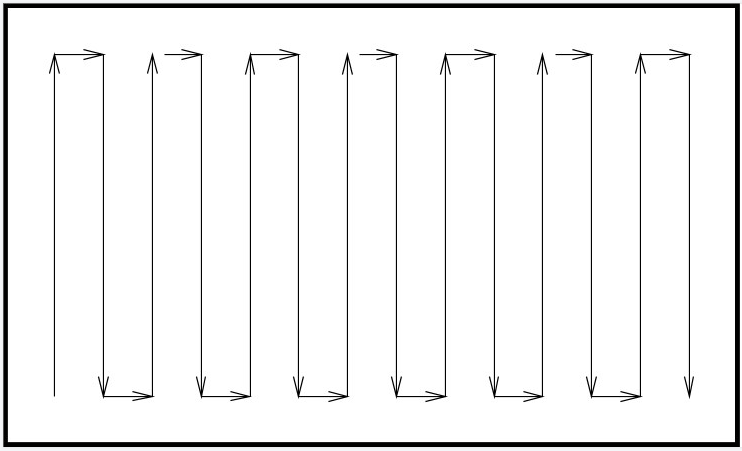
\includegraphics[width=6cm,height=4cm]{RS_Report/bcd.png}
\caption{BCD}
\label{bcd}
\end{minipage}
\begin{minipage}[t]{0.48\textwidth}
\centering
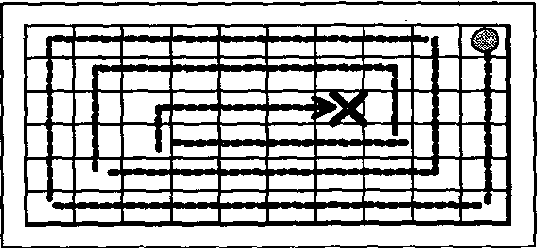
\includegraphics[width=6cm,height=4cm]{RS_Report/BSA.png}
\caption{BSA}
\label{bsa}
\end{minipage}
\end{figure}

\section{Implementation}
The individual functions and algorithms required during the experiments were tested separately and a map environment (with obstacles) was developed for the experiments.
\subsection{Map}
In this experiment, the path planning for the E-punk mobile robot starts with obtaining environmental information and establishing an environmental map. A reasonable representation of the environment facilitates the selection of a suitable search algorithm and ultimately achieves a good path with less time overhead. There are various methods to build the environment map, and this experiment mainly uses the raster method\cite{moravec1985high} to build the environment map in a static environment.This method is used because it decomposes the environmental space into local cells and describes the state of the environment in terms of whether obstacles occupy them or not. The maps produced by this method provide accurate metric information and are easier to understand and process than other methods.\\
A 90mm$\times$90mm map(see Fig.\ref{fig1}) was designed in Webots, which contained the obstacles. Since the CPP algorithm for the final comparison was built on a known map environment, in order to be able to tell the E-punk robot about this map, the built map was converted into a static  11$\times$11 raster map(see Fig.\ref{fig2}), where the value of the area within the array corresponding to the area where the map boundary and the obstacle are located was set to 1 and the value of the remaining freely movable area was set to 0.

\begin{figure}[htbp]
\centerline{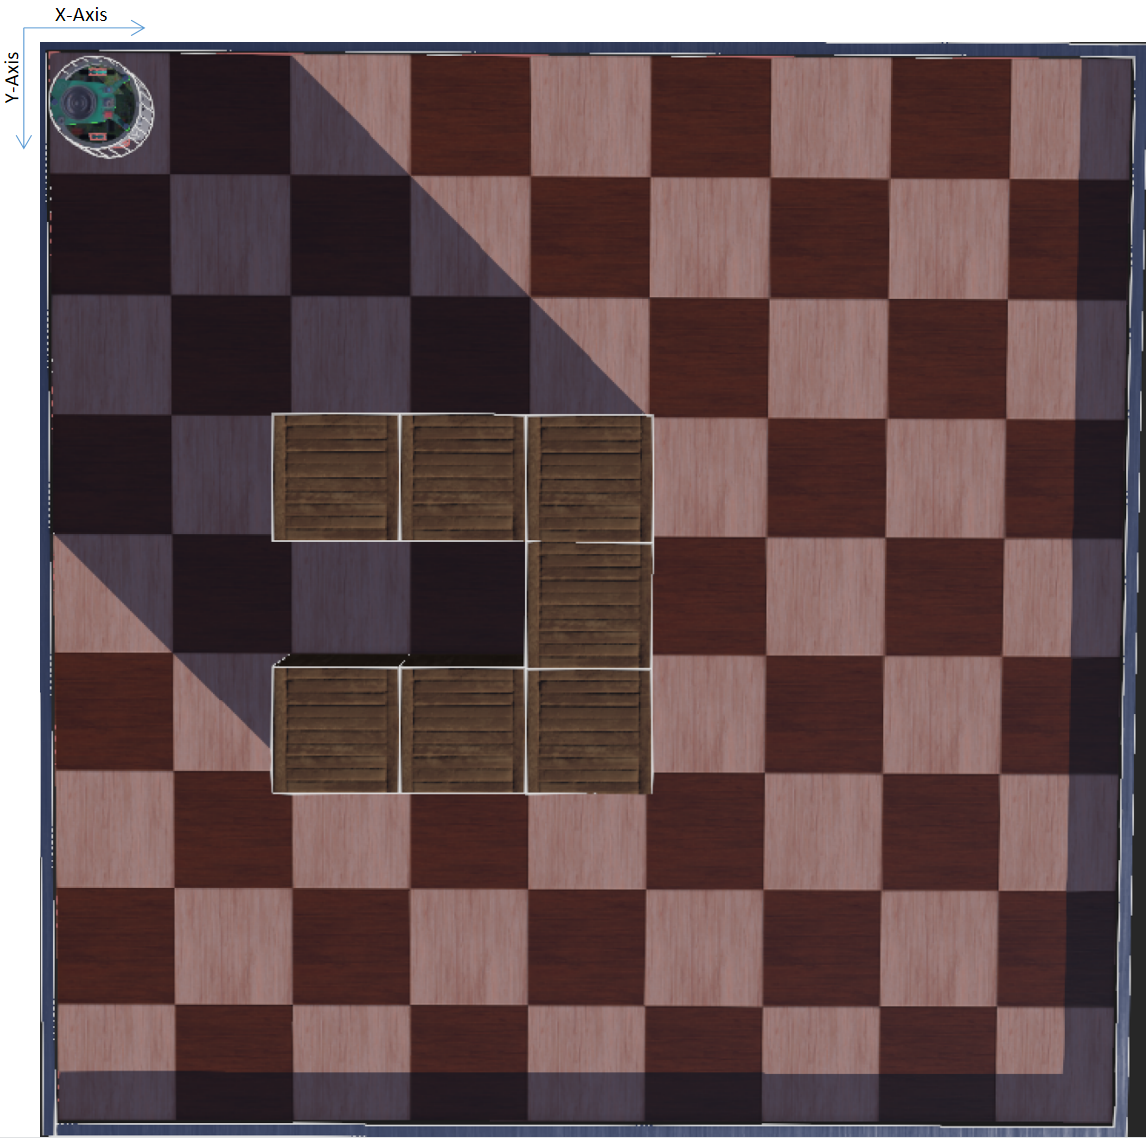
\includegraphics[scale=0.22]{RS_Report/Webots_map.png}}
\caption{E-punk campaign map built in Webots.}
\label{fig1}
\end{figure}

\begin{figure}[htbp]
\centerline{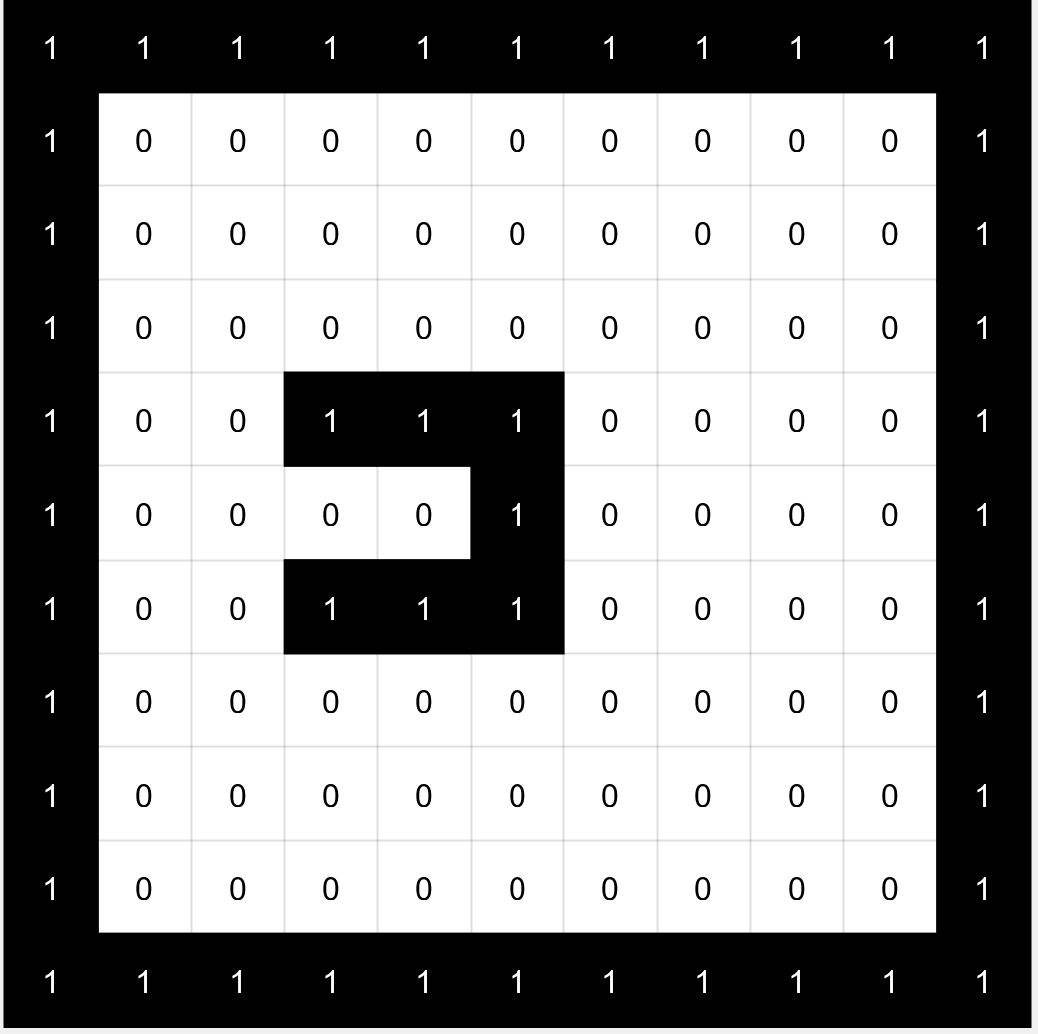
\includegraphics[scale=0.7]{map.png}}
\caption{Raster environment map built for E-punk.}
\label{fig2}
\end{figure}

\subsection{Odometry}

The odometry measures the initial to the final position of a mobile robot and is used in this experiment to localise and navigate the E-punk robot. The real E-punk robot uses stepper motors, which have been simulated in Webots. The angular increments of the left and right wheels during the robot's movement can be obtained using the simulated position sensors. Therefore, a global coordinate system is defined(see Fig.\ref{fig1}), and the kinematic calculation\cite{dudek2010computational} is used to obtain the position of the E-punk on this global coordinate system, where the position rotation angle theta is defined as the clockwise angle to the x-axis.\\
In the CPP algorithm used for this experiment, the E-punk robot must know its position and run the appropriate trigger conditions. By matching the coordinates calculated from the odometry with the position subscripts of the raster map matrix, the constructed raster map can be combined with the generated global coordinate system, thus mapping the robot's motion poses onto the constructed map and enabling the robot's motion.

\subsection{A* algorithm}
The sweeper robot returns to the initial point to recharge after completing the cleaning task in the real world. In this experiment, the robot is set to return to its initial position after completing the CPP task, which is designed to simulate the realistic motion of the robot better. The A* algorithm\cite{hart1968formal} is used to return to the initial position more quickly and with the shortest path.\\
As E-punk traverses the map, there will always be places that it has not traversed in a single loop. In this case, the experiment uses the A* algorithm to move the cart to the nearest untraversed region until the entire map is traversed.\\
The core of the a* algorithm is
\begin{equation}
    f(n) = g(n) + h(n)
\end{equation}
where $f(n)$ is the combined priority of node n. When the next node to be traversed needs to be selected, the algorithm always picks the node with the highest combined priority (smallest value). $g(n)$ is the cost of node n from the starting point. $h(n)$ is the expected cost of node n from the end point, which is the heuristic function of the A* algorithm.\\
The traversal direction is simplified in this experiment to match the raster map and speed up the calculation. The mobile robot can only move in four directions, up, down, left and right, in which case the heuristic function is calculated using the Manhattan distance method(see Fig.\ref{fig3}).

\begin{figure}[htbp]
\centerline{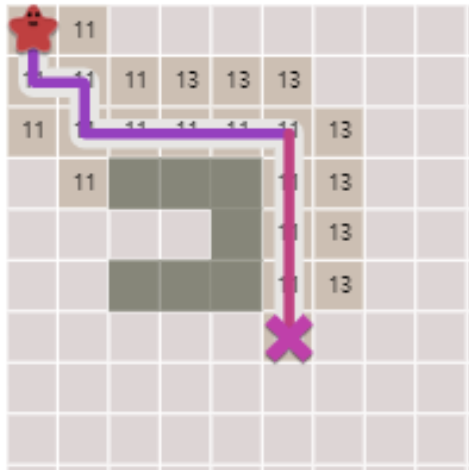
\includegraphics[scale=0.45]{RS_Report/astar.png}}
\caption{A* algorithm demonstration(the value in the cell is the value of $f(n)$).}
\label{fig3}
\end{figure}

\subsection{CPP algorithm}
 Fig.\ref{fig4} shows the overall form of the algorithm architecture combining the map, odometer, a* algorithm and CPP algorithm. The architecture allows E-punk to complete the map traversal and compare the completion times of the different CPP algorithms.
\subsubsection{Boustrophedon decomposition}
\subsubsection{Spanning tree covering}
\begin{figure}[htbp]
\centerline{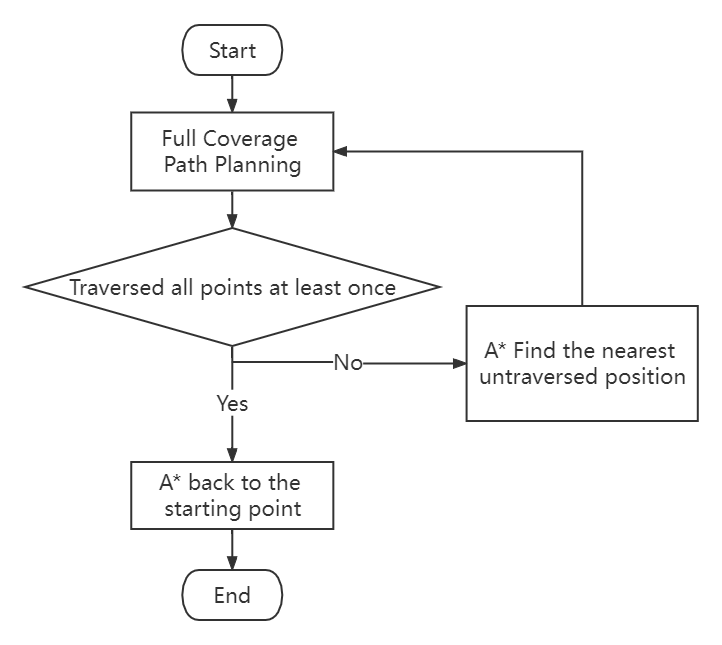
\includegraphics[scale=0.35]{RS_Report/RS_Report (1).png}}
\caption{Overall architecture of the CPP algorithm.}
\label{fig4}
\end{figure}


\section{Experiment Methodology}

\subsection{Overview of Method}
This experiment compares the completion times of two path planning algorithms, BCD and BSA, on the same map. Because the maps selected for the experiment were raster maps, all maps used for this experiment defined a cell size of 10mm$\times$10mm, and this area was scattered across the raster map. The experiment first verified whether the number of turns would directly affect the completion time. In this validation experiment, a60mm$\times$100mm map was created. This map was blank and was obstacle-free. By changing the orientation of the E-punk in the initial state, its turn position and number of turns during the map traversal became different. Compare the processing times of the two algorithms in these two different cases and complete this verification.\\
After concluding the validation experiment, the task completion times of the two path planning algorithms mentioned above were compared in different environments. The overall layout of the room on the floor for the robot vacuum cleaner does not usually change significantly except for the movement of people, so in this experiment, all maps are static maps, and obstacles do not move. This section is the central part of the experiment. A 90mm$\times$90mm map is defined, and 10mm$\times$10mm square obstacles are placed at random locations on the map. After the map is constructed, the performance of the two path planning algorithms is compared. After the comparison was completed on one map, the position of the obstacles was changed, and the same comparison experiment continued. This approach aims to reduce the impact of random errors in path planning caused by the particular location of some map obstacles. The experiments all started at the global coordinate system $(x, y, \theta) = (0, 0, 0)$, which in the simulated map is located in the top left corner of the map (see Fig.\ref{fig1}). Because the Webots simulation software comes with a time counter, the completion time is output when the simulation of both path algorithms ends. Webots is a simulator, and the experiment does not need to reduce random errors by recording times over multiple experiments. During the E-punk's movement, the coordinates of the locations it travels are recorded in real-time, and the set of path coordinates, which is used to visualise the route, is exported when the task is completed.

\subsection{Discussion of Variables}


\subsection{Discussion of Metric(s)}

 In this section you should discuss the rationale (why) you have selected your metric(s) - e.g. how do these metrics help us to interpret your results?  Your metric(s) will need to be applied consistently throughout your experiment for them to provide a comparison of performance.  
 
 You should discuss the advantages and disadvantages of your metric(s).  Often, we need more than one metric to compensate for the information which is confused or hidden in another metric.  By using more than one metric, we can get closer to the truth of the outcome of your experiment.  

\section{Results}

In this section you should present your results.  In general, it is best to aim for both \emph{quantitative} results (e.g., data) and \emph{qualitative} results (e.g., a written observation or graphic which is representative).  

You should use subsections where they aid in clarity.  For instance, it may be useful to present results for a "baseline" system, then a results for an "improved" system, and then finally results which consider both "baseline" and "improved" systems together.  However, this will depend entirely on your project and how you have designed your experiment.

When presenting results, aim for a presentation which clearly communicates an insight. For example, a large table of all the individual data requires the reader to do a lot of work to find out what is important.  In contrast, a table which appropriately presents the mean and standard deviation has summarised the results for the reader (and would be more useful).  Similarly, aim to combine data onto a chart when possible so that a direct comparison can be made - and when possible, include error bars.  


Remember to label all axis, caption all graphs, figures and tables, and to reference these elements in the report text (e.g. see figure \ref{fig1}) - never require a reader to have to come to their own conclusion or understanding, explain what they are looking at.  Remember to attempt to give an explanation for any anomalies in your results.  


\section{Discussion and Conclusion}

Begin your discussion and conclusion by re-stating your hypothesis.  You can literally copy-and-paste your hypothesis here.  

Because the VL1680X has been identified as an active sensor with ... limitations, we hypothesised that:
\begin{quote}
    by applying ... filtering to the sensor, we predict a measurable improvement of the sensor under ... conditions.  
\end{quote}

Make a discussion of what your results showed - whether this supported or refuted your hypothesis.  It may be that the results were mixed (supporting and refuting) and you should discuss that here. In your discussion, use this as another opportunity to demonstrate/evidence your understanding. Try to avoid stating the obvious - instead, use analysis/evaluation/synthesis to show that you understand \emph{how} and \emph{why} you saw the results you did.  What are the implications of your findings?  

This is also a good opportunity to evaluate your experiment and project as a whole.  You may wish to further discuss the limitations of the study (e.g. the difficulty of controlled/dependent variables, or any problems you faced in your project).  You may wish to make a recommendation for future work - but ensure that this is a clear advancement from the understanding you have gained and not wild speculation.


\bibliographystyle{ieeetr} 
\bibliography{biblio}


\end{document}
